\subsection{Systemets funktioner}
I det f�lgende punkt er systemets funktioner beskrevet ved Use Case-teknikken. Diagrammet nedenfor giver overblik over systemets funktioner.

\subsubsection{Use Case diagram}

\begin{figure}[h]
\centering
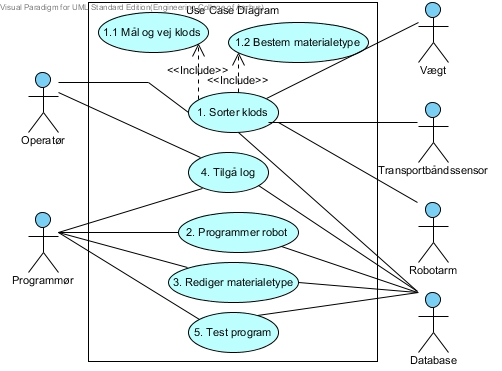
\includegraphics[scale=0.6]{Use_Cases/Diagrammer/Use_Case_Diagram.jpg} 
\caption{Use Case diagram}
\end{figure}

Systemets hovedfunktion er at sortere klodser efter matrialetype. Klodserne transporteres p� transportb�ndet, hvor en robotarm samler dem op og placerer dem i en kasse svarende til deres matrialetype.\\
Det er muligt for programm�ren at �ndre i robottens program via en PC.
\\\\
De forskellige Use Cases er detaljeret beskrevet senere i dokumentet, i afsnittet \textit{3 Funktionelle krav - Use Cases}
\subsection{Systemets begr�nsninger}
I produktopl�gget er et kamera beskrevet. I det endelige produkt er dette erstattet af en optisk sensor, som indg�r i styringen af transportb�ndet. Dette er foretaget efter aftale med kunde.\\
Den manuelle pendant er desuden fjernet, og i stedet kan robotten programmeres via et user interface p� en PC.

\subsection{Brugerprofil}
Det forventes at den administrative del, kun opereres af en person, som er orienteret i funktionerne for denne del af systemt.
\begin{itemize}

\item Brugeren \\
Brugeren er en prim�r akt�r af systemet. Det er ikke essentielt at denne person har nogen forst�else for, hvad der foreg�r bag systemet. Det eneste krav der stilles til brugeren er, at personen skal tilg� systemet fra en android platform.
\item Administrator \\
Administratoren er en prim�r akt�r af systmet. Det er ikke essentielt at denne person har forst�else for, hvordan en database virker. Det er dog vigtigt at personen er tr�net i at bruge denne del af systemet, og har en forst�else for, hvad de �ndringerne der foretages, g�r. Da administratoren bliver pr�senteret for et r�kke v�rkt�j, skal personen ikke n�dvendigvis have specielle kompetencer.

\end{itemize}


\subsection{Krav til udviklingsforl�bet}
Selvom der ikke blev vedlagt mange obligatoriske krav til dette projekt, er der i gruppen blevet fastlagt nogle udviklingsm�ssige rammer, som vil blive fulgt:

\subsubsection{Obligatoriske udviklingsv�rkt�jer}
Programmeringssproget skal i dette projekt v�re C\#, hvor der skal g�res brug af WPF til det grafiske interface samt .NET 4.0 frameworket. Til persistente data skal der g�res brug af SQL databaser, herunder logning og lagering af data fra klodserne. Undervejs i projektet udarbejdes to store dokumenter, en processrapport og et designdokument. \\

\subsubsection{Gruppedefinerede udviklingsv�rkt�jer}
Til selve udviklingen er der blevet valgt at f�lge v�sentlige principper fra Scrum frameworket. Der blev gjort brug af dette i tredje semesterprojektet, hvor det blev set som ganske brugbart. Herunder blev der ogs� gjort brug af nogle af Extreme Programming-principperne. \\ 




\subsection{Foruds�tninger}
Det forventes at der kan skabes en l�bende kommunikation med kunden (Michael Alr�e, ma@iha.dk). Hertil vil der l�bende blive holdt m�der, hvor �ndringer diskuteres.
